\chapter{Interface d'alimentation}
		
Afin de fonctionner dans son intégralité, le système a besoin de 
différents niveaux de tension, parmi lesquels un niveau de 5V pour 
le servomoteur de direction, et du 3.3V pour l'alimentation des 
microcontrôleurs et pour l'utilisation du 
\textit{Bluetooth Low Energy}. 
Il est donc prévu de concevoir à cet effet un PCB permettant 
d'obtenir tous les niveaux de tension nécessaires sur une seule 
carte et ainsi les distribuer à tous les éléments fonctionnels du 
système. 
	
Après une caractérisation de la batterie utilisée, nous présenterons 
la mise en oeuvre des conversions tension source vers 5V, puis 5V 
vers 3.3V, pour enfin présenter la carte électronique d'interface	 
d'alimentation.
		
	\section{Caractérisation de la source d'alimentation}
			
	La source d'alimentation de notre projet est une 
	\textbf{batterie LiPo 3S}. Quelques généralités sur les batteries 
	LiPo et leur utilisation seront exposées dans un premier temps. 
	Nous mettrons ensuite en oeuvre un modèle \textit{PSIM} de la batterie
	considérée avant d'en vérifier les caractéristiques en simulation. 
	Finalement, nous proposerons un montage de protection contre la 
	sous-tension batterie, pouvant être destructrice pour ce type de 
	batterie.
		
		\subsection{Généralités sur les batteries LiPo}
			
		Ce type de batterie est structuré par 3 cellules LiPo de 3.7V en 
		série, soit une \textbf{tension nominale de 11.1V} (3 x 3.7V) pour 
		la batterie LiPo 3S à vide. Un élément LiPo est en fait une batterie 
		Li-ion où l'électrolyte est un polymère gélifié.
			
		Il est à garder en mémoire que \textbf{la décharge d'un élément LiPo 
		en-dessous de 2.5V entraîne sa destruction}. De manière générale, il 
		est recommandé de 
		\textit{ne pas décharger les éléments en-dessous de 3.3V} 
		si l'on souhaite une durée de vie optimale pour ce type de batterie.
		Nous tiendrons compte de cette contrainte par la suite lors de la
		mise en oeuvre d'un circuit de protection contre la sous-tension. 
			
		A l'inverse, chaque élément LiPo 
		\textbf{ne doit jamais être chargé au-dessus de 4.2V}, au risque de 
		provoquer un \textbf{possible incendie}. Dans le cas d'une batterie 
		constituée d'éléments LiPo multiples, il est 
		\textbf{impératif d'utiliser un \textit{égaliseur}} dans le circuit 
		de charge. Cet égaliseur est de manière générale disponible sur tous
		les chargeurs standards de batteries LiPo.
		
		% Source : http://geeby22.over-blog.com/page-4287873.html
			
		\subsection{Modélisation de la batterie LiPo}
			
		La batterie LiPo utilisée pour notre système va être modélisée sous 
		\textit{PSIM} par l'élément Li-Ion Battery comme montré en 
		\textsc{Figure \ref{lipo_model_psim}}.
			
		\begin{figure}[ht]
			\begin{center}
				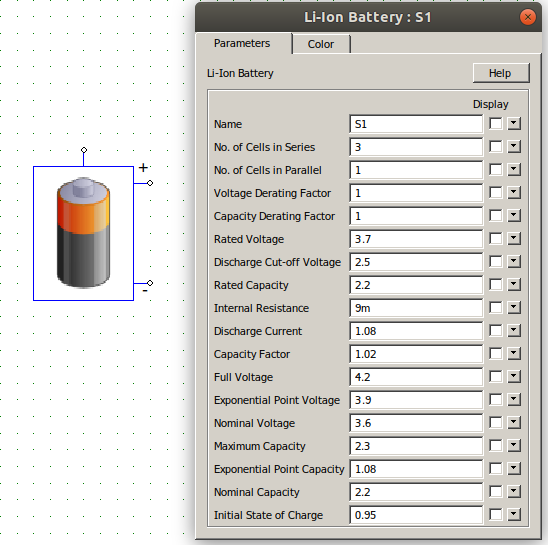
\includegraphics[scale=0.5]{../Illus/lipo_model_psim.png}
			\end{center}
			\caption{Élément \textit{PSIM} modélisant la batterie LiPo du 
			système}
			\label{lipo_model_psim}
		\end{figure}
			
			\subsubsection{Caractéristiques principales de la batterie utilisée}
			
			La \textsc{Table \ref{carac_lipo_psim}} met en avant les 
			caractéristiques principales du modèle de la batterie utilisée.
			
			\begin{table}[h]
				\begin{center}
					\begin{tabular}{l c}
						\textbf{Paramètre}		& \textbf{Valeur}	\\
						\hline
						Nombre de cellules 		& 3 				\\
						Capacité nominale		& 2200mAh 			\\
						Capacité maximale		& 2300mAh			\\
						Résistance interne		& 9m$\Omega$		\\
					\end{tabular}
				\end{center}
				\caption{Caractéristiques principales du modèle \textit{PSIM} de la batterie}
				\label{carac_lipo_psim}
			\end{table}
			
				\vspace{-0.5em}
			
				\paragraph{Nombre de cellules}
				
				La batterie considérée comportant 3 cellules, nous pouvons ainsi
				déterminer ses tensions caractéristiques, à savoir :
				\begin{itemize}
					\item[$\bullet$] une tension nominale de 11.1V (3 x 3.7V) ;
					\item[$\bullet$] une tension maximale de 12.6V (3 x 4.2V) ;
					\item[$\bullet$] une tension minimale d'utilisation de 9.9V (3 x 3.3V). 
				\end{itemize}
				
				\vspace{-0.5em}
				
				\paragraph{Capacité nominale}
				
				Elle correspond à la \textit{taille du réservoir d'énergie} que 
				constitue la batterie. Bien que des capacités de batterie plus
				élevées soient synonymes de meilleurs temps d'autonomie, il en
				résulte dans le même des batteries plus lourdes et volumineuses
				pouvant allourdir la structure de l'aéroglisseur.
				Une capacité de 2200mAh est alors un bon compromis en plus d'être
				une valeur courante sur le marché.
				
				\vspace{-0.5em}
			
				\paragraph{État initial de charge}
			
				Nous considèrerons pour nos simulations un 
				\textbf{état initial de charge de 95\%}, 
				valeur raisonnable correspondant à la réalité d'une 
				batterie chargée.
			
			%\subsubsection{Vérification des caractéristiques du modèle}
			
			%cf. tuto \cite{LiPo_PSIM}
			
		\subsection{Protection contre la sous-tension batterie}
			
		Nous avons vu dans les généralités sur les batteries LiPo que la 
		sous-tension pouvait être destructrice pour ce type de batterie. 
		Cependant, lors de l'utilisation de l'aéroglisseur, il faudra faire
		attention à surveiller régulièrement la tension source afin de ne 
		pas descendre en-dessous d'une valeur de tension critique pour la 
		batterie. 
		Un système électronique de détection et de coupure du système à 
		partir d'un certaine tension de décharge de la batterie peut 
		solutionner cette problématique. Nous mettrons ici en oeuvre un tel 
		circuit, dénommé \textit{Under-Voltage FeedBack} (\textit{UVFB}).
			
			\subsubsection{Généralités sur le circuit UVFB}
				
			Le montage typique d'un circuit UVFB est exposé en Figure 
				
			\begin{figure}[h]
				\begin{center}
					\begin{circuitikz}
					\draw
					(0,5) 	to [V, l=$V_{BAT}$] (0,0)
					(0,5)	to (2,5) 
							to [R, l=$R_1$] (2,3) to (2,2)
							to [R, l=$R_2$] (2,0) to (0,0)
					(2,5)	to [short, *-*] (4,5)
							to [R, l=$R_3$] (4,3)
							to [short, -*]	(6,3)
					(6,0)   to [thyristor, n=TL, l_=TL431]  (6,3)
					(2,0)	to [short, *-*] (6,0)
							to [short, -*]  (8,0)
					(2,2.2)	to [short, *-]  (TL.G)
					%(6,5) node [pmos, rotate=90] {Q1};
					(6,5) node[pfet,bodydiode,rotate=90](Q1){}
					(6,3) to (Q1.G) (Q1.S) to (4,5) (Q1.D) to [short, -*] (8,5);
					\draw[black,thick,-latex] (8,0.2) -- (8,4.8) node [right,midway] {$V_{P}$};
					\end{circuitikz}
				\end{center}
				\caption{Montage typique d'un circuit \textit{Under-Voltage FeedBack}}
			\end{figure}
				
			\subsubsection{Dimensionnement des composants}
				
			Nous allons devoir dimensionner les composants du montage ci-dessus
			de manière à répondre à la problématique particulière de notre 
			système. 
			La première étape de fixer les valeurs des résistances afin 
			d'obtenir la tension de coupure 
	
	\newpage		
			
	\section{Conversion tension batterie vers 5V}
			
	L'alimentation du servomoteur de direction nécessite d'obtenir un 
	niveau de tension de 5V à partir de la tension 11.1V standard de la 
	batterie LiPo 3S. 
	Pour cela, nous avons mis en oeuvre le régulateur à découpage 
	\textbf{LM22672MR-5.0/NOPB} du constructeur 
	\textit{Texas Instruments}. 
	Ce régulateur permet d'implémenter un convertisseur de type Buck 
	en utilisant un minimum de composants externes. 
	Toutefois, ces derniers devront être correctement dimensionnés afin 
	de prendre en compte les contraintes de la source et de la charge.
	
	Nous exposerons dans un premier temps les généralités sur le composant
	\texttt{LM22672} avant d'en proposer un modèle \textit{PSIM} complet. 
	Ce modèle nous permettra de vérifier le dimensionnement des composants
	extérieurs au régulateur à découpage et de valider la mise en oeuvre
	du circuit complet. Finalement, nous prendrons en compte les aspects
	thermiques du circuit avant de proposer un routage du convertisseur.
			
		\subsection{Généralités sur le composant LM22672}
		
		Le composant \texttt{LM22672} est un régulateur proposant toutes 
		les fonctionnalités permettant d'implémenter un convertisseur 
		Buck performant \cite{LM22672}. Il est disponible en deux versions 
		de tension de sortie :
		\begin{itemize}
			\item[$\bullet$]	\texttt{-ADJ} à tension réglable jusqu'à un minimum
							 	de 1.285V ;
			\item[$\bullet$]	\texttt{-5.0} à tension de sortie fixe 5V.			 
		\end{itemize}
		Nous retiendrons dans notre cadre d'application la seconde version
		nous permettant d'obtenir facilement un niveau de tension 5V.
			
			\subsubsection{Caractéristiques électriques du composant}
			
			La documentation technique du composant nous permet d'accéder aux
			caractéristiques électriques importantes du composant. Elles sont
			synthétisées dans la \textsc{Table \ref{carac_elec_lm22672}}.
			Les caractéristiques y sont données pour la version \texttt{-5.0}
			du composant.
			
			\begin{table}[h]
				\begin{center}
					\begin{tabular}{|l l | r r r | c|}
					\hline
					\multicolumn{2}{|c|}{\textbf{PARAMETER}}	& \textbf{MIN}	& \textbf{TYP}	
																& \textbf{MAX}	& \textbf{UNIT}\\
					\hline
					$V_{FB}$		&	Feedback Voltage		& 4.925	&	5.0	& 5.075	&	V			\\
					\hline
					$R_{DS(ON)}$ 	& 	Switch On-Resistance 	&		&	0.2	&  0.32	&	$\Omega$	\\
					\hline
					$F_{SW}$		&	Oscillator Frequency	&	400	&	500	&	600	&	kHz			\\
					\hline
					$T_{OFF}$		&	Minimum Off-time		&	100	&	200	&	300	&	ns			\\
					\hline
					$T_{ON}$		&	Minimum On-time			&		&	100	&		&	ns			\\
					\hline
					$I_{SS}$		& 	Soft-Start Current		&	30	&	50	&	70	&	$\mu$A		\\
					\hline
					$T_{SD}$		& 	Thermal Shutdown Threshold	&	&	150	&		&	\degre C	\\
					\hline
				\end{tabular}				
				\end{center}	
				\caption{Caractéristiques électriques du convertisseur \texttt{LM22672} \cite{LM22672}}
				\label{carac_elec_lm22672}
			\end{table}
			
			Ces différentes caractéristiques vont nous être utiles pour pouvoir 
			modéliser au mieux les différentes fonctions du composant et ainsi
			en proposer un modèle le plus fidèle possible.
		 
			\subsubsection{Entrées et sorties du composant}
			
			Les entrées et sorties du convertisseur \texttt{LM22672} sont répertoriées dans la
			\textsc{Table \ref{io_lm22672}}. 
			Une bonne connaissance de ces entrées et sorties ainsi que de leur 
			utilité permettra une meilleure approche lors de la modélisation 
			du composant.
			
			\begin{table}[h]
				\begin{center}
					\begin{tabular}{|l|c|c|l|l|}
					\hline
					\textbf{NOM}	& \textbf{NO.}	& \textbf{TYPE}	& \textbf{DESCRIPTION}	& \textbf{FONCTIONNALITÉS} \\
					\hline										
					BOOT			&	1			& 	Entrée		& 	Entrée de bootstrap	&	Accès au 
																								potentiel de la 
																								\textit{gate} du NFET	\\
					EN				&	5			&	Entrée		& 	Mise en marche		& 	Contrôle de
																								l'allumage du régulateur\\
					EP				& 	EP			&	-			&	Pad externe			& 	Connection thermique 
																								masse - PCB 			\\
					FB				&	4			&	Entrée		&	Entrée de feedback	&	Entrée de rétroaction
																								du régulateur			\\
					GND				&	6			&	-			&	Masse du régulateur	&	Connection vers la masse 
																								du régulateur			\\
					RT/SYNC			&	3			&	Entrée		&	Mode d'oscillation	&	Ajustement de
																								l'oscillateur interne	\\
					SS				&	2			&	Entrée		&	Entrée de soft-start&	Modification du temps
																								de soft-start			\\
					SW				&	8			&	Sortie		&	Sortie de découpage	&	Sortie du régulateur à
																								découpage				\\	
					VIN				&	7			&	Entrée		&	Tension d'entrée	&	Tension d'entrée et
																								d'alimentation			\\
					\hline
				\end{tabular}				
				\end{center}	
				\caption{Entrées et sorties du convertisseur \texttt{LM22672} \cite{LM22672}}
				\label{io_lm22672}
			\end{table}
			
			\subsubsection{Schéma d'application standard}
				
			Le montage standard de mise en oeuvre d'un régulateur à découpage
			à base du composant \texttt{LM22672} est montré en 
			\textsc{Figure \ref{buck_gen_scheme}}. Il présente notamment les
			composants externes qui seront à dimensionner afin d'obtenir le
			fonctionnement désiré pour notre application.
			
			\begin{figure}[h]
				\begin{center}
					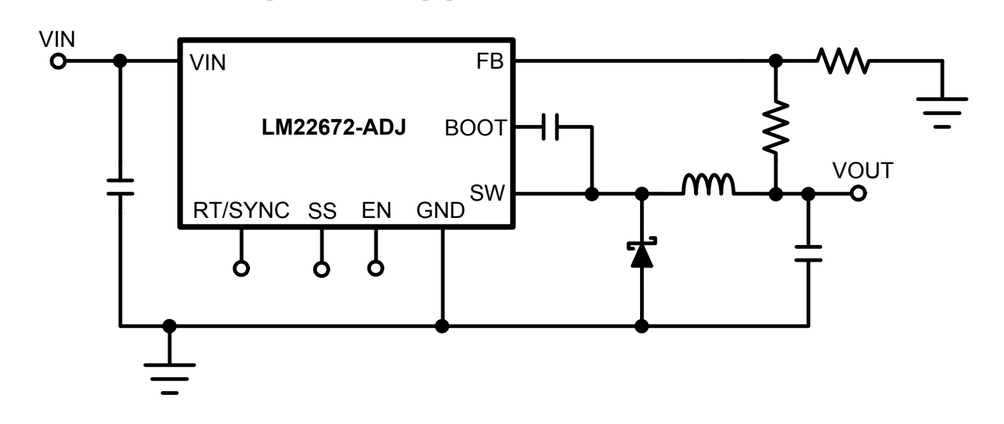
\includegraphics[scale=0.5]{../Illus/buck_gen_scheme.png}
				\end{center}
				\caption{Schéma d'application standard du composant \texttt{LM22672}}
				\label{buck_gen_scheme}
			\end{figure}
				
		\subsection{Modélisation du composant LM22672}
			
		Afin de pouvoir établir un modèle fidèle du composant 
		\texttt{LM22672}, nous allons nous baser sur le diagramme bloc
		fonctionnel donné dans la datasheet du constructeur 
		\cite{LM22672} et représenté en
		\textsc{Figure \ref{func_bloc_lm22672}}. 
		
		Nous allons identifier chaque bloc et le modéliser le plus 
		adéquatement possible en accord avec les indications de la datasheet. 
		
		Ces différents blocs seront ensuite assemblés afin d'obtenir le modèle 
		complet du composant. Ce modèle sera finalement implémenté dans le 
		logiciel \textit{PSIM} et associé avec tous les composants externes 
		afin de vérifier le bon dimensionnement de ces derniers.
								
		\begin{figure}[h]
			\begin{center}
				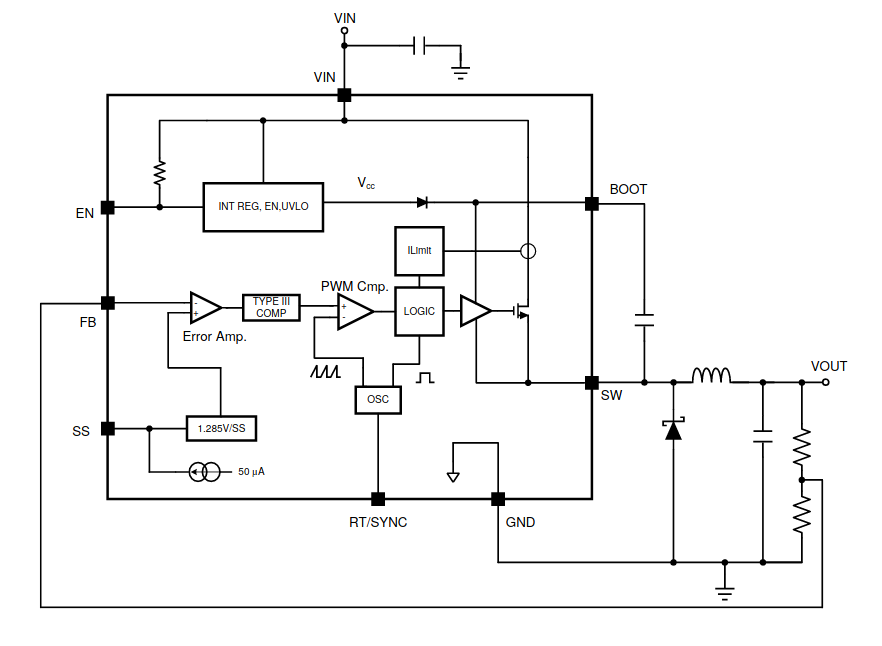
\includegraphics[scale=0.4]{../Illus/func_bloc_lm22672.png}
			\end{center}
			\vspace{-2em}
			\caption{Diagramme bloc fonctionnel du LM22672 tiré de la datasheet \cite{LM22672}}
			\label{func_bloc_lm22672}
		\end{figure}
				
			\subsubsection{Modélisation de la fonctionnalité Soft-Start}
			
			La fonctionnalité de soft-start (SS) permet au régulateur 
			d'atteindre la valeur finale de sortie progressivement en
			limitant les oscillations ou perturbations liées au démarrage.
			
			En effet, les convertisseurs de type Buck ont tendance à
			présenter au démarrage un courant d'appel important mais
			aussi des dépassements en tension. Ces phénomènes peuvent
			se traduire en des pertes en commutation conséquentes.
			
			En effet, au démarrage du convertisseur la tension de sortie
			doit varier de 0V vers la tension finale désirée 
			(5V dans notre cas), provoquant une forte différence en tension
			au niveau de l'amplificateur d'erreur et engendrant par conséquent
			un très haut rapport cyclique (proche de 100\%). 
			Cependant, un rapport cyclique de 100\% peut impliquer un fort appel
			en courant au niveau de l'inductance de sortie. Ce courant circule 
			toutefois encore un certain moment du fait que le courant à travers 
			une inductance ne peut être discontinu. Cet appel en courant est
			indésirable et peut même endommager le convertisseur 
			\cite{Soft_Start}.
			
			\begin{figure}[h]
				\begin{center}
					\begin{circuitikz}
						\draw
						(0,0)		node [ground] {}
									to [C, l=$C_{SS}$] 	(0,1.5)
									to (0,2.5)
						(0,4.5)		node [vcc] {$V_{CC}$}
									to [I, l_=$I_{SS}$] (0,2.5)
						(2,1.5)		to [V, l=$V_{REF}$]	(2,0.0)	
									node [ground] {}
						(2,2.5)		node [adder] (add) {}
						(add.1)		to [short, -*] (0,2.5)
						(add.1)		node [inputarrow]  {}
						(add.2)		to (2,1.5)
						(add.2)		node [inputarrow, rotate=90]  {}
						(5,3.0)		node [op amp] (opamp) {}
						(opamp.+)	to (add.3)
						(opamp.-)	to [short, -o] (3,3.5)
									node [left] {$V_{FB}$}	
						(opamp.up)	node [vcc] {$V_{CC}$}
						(opamp.down)node [ground] {}
						(8,2.5)		node [op amp] (opamp2) {}	
						(opamp2.-)	to (opamp.out)
						(opamp2.+)	to (6,2.0)
									to [short, -o] (6,1.5)
									node [below] {\textit{Oscillateur}}	
						(opamp2.out)to [short, -o] (10,2.5)
									node [right] {\textit{Vers NFET}}
						(opamp2.up)	node [vcc] {$V_{CC}$}
						(opamp2.down)	node [ground] {}
						(9,4.0)		node [above] {Comparateur PWM};
					\end{circuitikz}
				\end{center}
				\vspace{-1em}
				\caption{Montage standard d'un soft-start mettant en oeuvre une \textit{Pulse Skipping Modulation}}
				\label{soft_start_scheme}
			\end{figure}
			
			Le circuit de soft-start, et notamment celui proposé en 
			\textsc{Figure \ref{soft_start_scheme}}, 
			permet d'éviter les phénomènes précédemment explicités.
			Un tel montage met en fait en oeuvre une 
			\textbf{Modulation du Saut d'Impulsion} 
			(MSI, en anglais \textit{Pulse Skipping Modulation} ou \textit{PSM})
			permettant de réduire les pertes en commutation et en améliorant
			l'efficacité d'un convertisseur de type Buck \cite{Soft_Start}.			  
			Il permet notamment d'éviter une augmentation trop brusque de la
			valeur du rapport cyclique lors du démarrage du convertisseur.
			
			La \textsc{Table \ref{carac_elec_lm22672}} nous indique que la 
			valeur de courant de soft-start $I_{SS}=50\mu$A est utilisée dans 
			la structure du composant \texttt{LM22672}.
			
			La capacité $C_{SS}$ constitue quant-à-elle un composant externe
			qui sera déterminé lors du dimensionnement des composants externes 
			au convertisseur (voir \textsc{Section~\ref{sec:dim_soft_start}}).
			
			\subsubsection{Modélisation de l'ajustement de la fréquence de découpage}
			
			Le convertisseur \texttt{LM22672} peut suivre trois modes différents
			de fonctionnement suivant l'action réalisée sur l'entrée 
			\texttt{RT/SYNC} :
			\begin{itemize}
				\item[$\bullet$]si l'entrée \texttt{RT/SYNC} est laissée flottante,
								alors la fréquence de découpage est fixée par
								defaut à 500kHz de manière interne au système ;
				\item[$\bullet$]si l'entrée \texttt{RT/SYNC} est reliée à la masse
								\textit{via} une résistance de valeur comprise entre 
								25 k$\Omega$ et 200 k$\Omega$, alors la fréquence de découpage
								peut être ajustée entre 1 MHz et 200 kHz ;
				\item[$\bullet$]si l'entrée \texttt{RT/SYNC} est reliée à un oscillateur
								externe, alors le convertisseur va fonctionner à la fréquence
								imposée sur l'entrée et le composant peut par exemple être
								synchronisé avec un autre \texttt{LM22672}.
			\end{itemize}
			
			Nous retiendrons dans notre cas la deuxième possibilité de 
			fonctionnement, permettant un réglage de la fréquence de découpage
			\textit{via} une résistance externe. C'est ce comportement que nous
			allons modéliser par la suite. 
			
			Nous allons notamment nous baser
			sur la courbe typique de fréquence de découpage en fonction de la
			valeur de la résistance externe $R_T$. Cette courbe est disponible
			dans la documentation technique du \texttt{LM22672} \cite{LM22672}
			et est également donnée en \textsc{Figure \ref{curve_freq_res}}.
			
			\begin{figure}[h]
				\begin{center}
					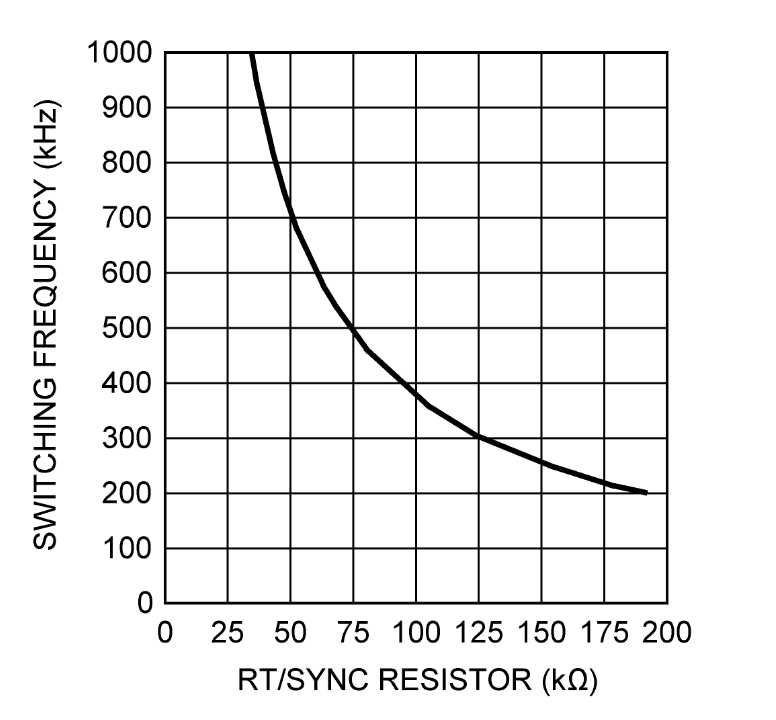
\includegraphics[scale=0.35]{../Illus/curve_freq_res.png}
				\end{center}
				\vspace{-1em}
				\caption{Courbe de la fréquence de découpage en fonction de la 
				résistance $R_T$ \cite{LM22672}}
				\label{curve_freq_res}
			\end{figure}
			
			Afin de modéliser cet oscillateur réglable, nous avons retenu la 
			structure à amplificateur opérationnel de la 
			\textsc{Figure \ref{osc_reg_scheme}}.
			
			\begin{figure}[h]
				\begin{center}
					\begin{circuitikz}
						\draw
						(0,0.0) 	node [ground] {}
									to [R, l=$R_2$] (0,2.5) to (0,3)
									to [R, l=$R_1$] (0,5.0)	
									node [vcc] {$V_{CC}$}
						(5,3.0)		node [op amp] (opamp) {}
						(0,2.5) 	to [short, *-] (opamp.+)
						(3,2.5)		to [short, *-] (3.0,1)
									to [R,l_=$R_3$](7.5,1)
									to [short, -*] (7.5,3)
									to [R,l_=$R_4$](7.5,5)
									node [vcc] {$V_{CC}$}
						(6.5,3)		to (6.5,5.5)
									to [vR,l_=$R_T$](3.0,5.5)
									to [short, -*]  (3.0,3.5) 
									to (opamp.-)
						(3.0,3.5)	to [C,l_=$C_1$] (1.0,3.5)
									node [ground, rotate=270] {}
						(opamp.out) to [short, -*] 	(6.5,3.0)
									to (7.5,3.0)
						(opamp.up)	node [vcc] {$V_{CC}$}
						(opamp.down)node [ground] {};  		
					\end{circuitikz}
				\end{center}
				\vspace{-1em}
				\caption{Schéma d'un oscillateur à amplificateur opérationnel
				réglable via $R_T$}
				\label{osc_reg_scheme}
			\end{figure}
			
			On fixera alors $R_1=R_2=R_3=100$k$\Omega$.
				
			\subsubsection{Modélisation du compensateur de type III}
				
				\paragraph{Généralités}
				
				Le composant LM22672 intègre dans sa structure un compensateur 
				de type III. Ce compensateur joue un rôle clé dans la stabilité 
				de la sortie notamment dans le cas des convertisseurs Buck comme
				c'est ici le cas. Certains montages Buck peuvent se satisfaire 
				d'un simple contrôleur PI 
				La structure générique d'un compensateur de type III est donnée 
				en \textsc{Figure \ref{comp_III_gen}}.
				
				\begin{figure}[h]
					\begin{center}
						\begin{circuitikz}
							\draw
							(0,0) 		node[op amp](opamp){}
							(opamp.-)	to [short, -*] 		(-1.5,0.5)
										to [short, -*] 		(-1.5,2.0)
										to [R, l=$R_{c1}$]	( 0.5,2.0)
										to [C, l=$C_{c1}$]	( 2.5,2.0)
							(-1.5,2.0)	to (-1.5,4.0)
										to [C, l=$C_{c2}$]	( 2.5,4.0)
										to [short, -*]		( 2.5,2.0)
										to [short, -*]		( 2.5,0.0)
										to (opamp.out)
							(-1.5,0.5)	to [short, -*]		(-3.5,0.5)
										to [R, l=$R_{f1}$]	(-3.5,4.0)
										to (-5.5,4.0)
										to [R, l=$R_{f3}$]	(-5.5,2.0)
										to [C, l=$C_{f3}$]	(-5.5,0.5)
										to (-3.5,0.5)
										to [R, l_=$R_{f2}$]	(-3.5,-2) node[ground]{};
						\end{circuitikz}
					\end{center}
					\caption{Structure générique d'un compensateur de type III \cite{AN1162}}
					\label{comp_III_gen}
				\end{figure}	
					
				On peut alors déduire de cette structure la fonction de transfert 
				(\ref{tf_comp_III}) du compensateur.
					
				\begin{equation}
					H(s) 
					= 
					-\frac{(1+s R_2 C_2)(1+s(R_1+R_3)C_3)}
					{sR_1(C_1+C_2)
					\left[1+sR_2\left(\frac{C_1C_2}{C_1+C_2}\right)\right]
					(1+sR_3C_3)}
					\label{tf_comp_III}
				\end{equation}
					
				La fonction de transfert (\ref{tf_comp_III}) peut être simplifiée 
				à partir de quelques considérations fréquentielles. En effet, pour 
				respecter la forme asymptotique attendue d'un Bode de compensateur 
				de type III (voir Figure), il faudra considérer le zéro généré par 
				$R_2$ et $C_2$ comme ayant une pulsation plus faible que le pôle 
				généré par $R_2$ et $C_1$. 
				Cela reviendra donc à négliger la valeur de $C_1$ devant celle de 
				$C_2$ ($C_1 << C_2$). 
				Par un raisonnement analogue, on considérera la valeur de $R_3$ 
				négligeable devant celle de $R_1$ ($R_3 << R_1$). 
				On déduit alors de ces considérations une nouvelle expression de 
				la fonction de transfert du compensateur.
					
				\begin{equation}
					H(s) \sim -\frac{(1+s R_2 C_2)(1+sR_1 C_3)}
					{sR_1 C_2 (1+sR_2 C_1) (1+sR_3C_3)}
					\label{tf_comp_III_simp}
				\end{equation}
					
				La fonction de transfert simplifiée (\ref{tf_comp_III_simp}) nous 
				permet finalement de conclure que le compensateur possède 
				\textbf{deux zéros} et \textbf{trois pôles} aux pulsations 
				respectives :
					
				\begin{equation}
					\omega_{Z1} = \frac{1}{R_2C_2}
					\quad\quad\quad
					\omega_{Z2} = \frac{1}{R_1C_3}
				\end{equation}
					
				\begin{equation}
					\omega_{P1} = 0
					\quad\quad\quad
					\omega_{P2} = \frac{1}{R_2C_1}
					\quad\quad\quad
					\omega_{P3} = \frac{1}{R_3C_3}
				\end{equation}
					
				Une synthèse de ces pulsations peut être faite sur le diagramme de 
				Bode montré en Figure 					
					
				\paragraph{Détermination des composants du modèle}
				
				Il est maintenant temps de déterminer les éléments particuliers 
				de ce compensateur dans notre cas d'application. Le compensateur 
				de type III inclus dans le composant LM22672 est caractérisé par 
				le diagramme de Bode en gain donné dans la section 
				\textit{Internal Loop Compensation} de la datasheet. Ce diagramme 
				de Bode est exposé en \textsc{Figure \ref{comp_gain}}.
										
				\begin{figure}[h]
					\begin{center}
						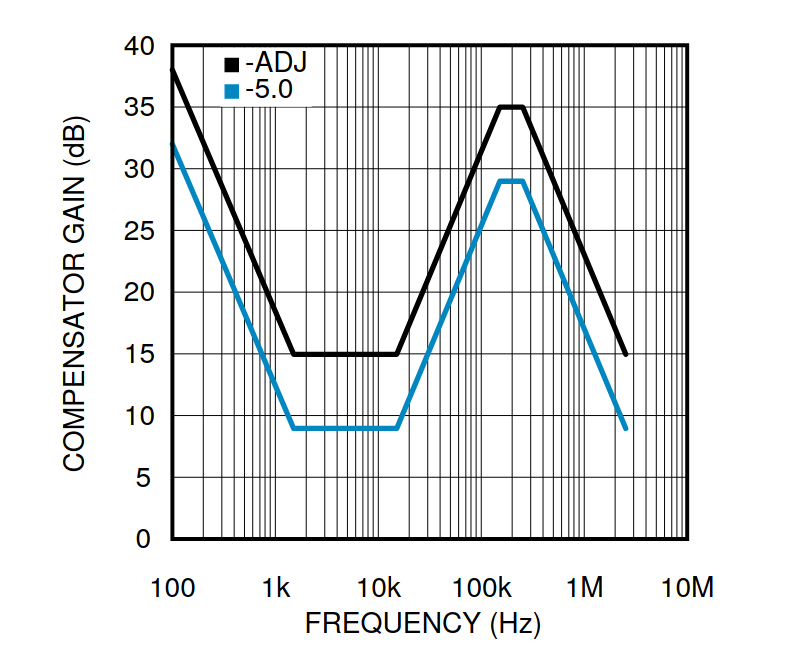
\includegraphics[scale=0.4]{../Illus/comp_gain.png}
					\end{center}
					\vspace{-2em}
					\caption{Bode en gain du compensateur de type III interne au LM22672 \cite{LM22672}}
					\label{comp_gain}
				\end{figure}
					
				La \textsc{Figure \ref{comp_gain}} nous permet de déterminer de 
				nombreuses informations sur le compensateur, et notamment les 
				valeurs des différentes fréquences de cassure du système. En accord
				avec l'allure typique d'un diagramme de Bode de compensateur de 
				type III donné en Figure , la lecture de la Figure nous permet de 
				déterminer les valeurs des zéros et pôles de la fonction de 
				transfert (). Les valeurs des zéros sont données en 
				(\ref{freq_III_zero}) et les valeurs des pôles sont données en 
				(\ref{freq_III_pole})
										
				\begin{equation}
					F_{Z1} = 
					\label{freq_III_zero}
				\end{equation}
				
				Il sera notamment à garder en mémoire lors de 
					
				\paragraph{Simulation fréquentielle}  
					
				\begin{figure}[h]
					\begin{center}
						\begin{tikzpicture}
							\begin{axis}[
								x=13mm,
								y=2mm,
								xmode=log,
								axis x line=middle,
								%axis y line=middle,
								xmin = 100, xmax = 10000000,
								ymin = 0, ymax=40,
								grid=both,
								xlabel=Fréquence (Hz),
								ylabel=Gain du compensateur (dB)]

								%\addplot[color=blue]
								%table[x={Frequency},y={amp(Vo1)}]
								%{data/bode_comp_III.txt};

								\addplot[color=orange]
								table[x={Frequency},y={amp(Vo1)}]
								{data/bode_comp_III.txt};
							\end{axis}
						\end{tikzpicture}
					\end{center}
					\label{bode_comp_III}
					\caption{Diagramme de Bode du compensateur de type III : 
					\textcolor{blue}{théorique} et 
					\textcolor{orange}{modèle PSIM}}
				\end{figure}
					
		\subsection{Dimensionnement des composants externes}
			
			\subsubsection{Capacité de soft-start}
			\label{sec:dim_soft_start}
			
			La documentation technique indique que ce temps de montée 
				
			L'équation approximative du temps de soft-start peut être estimé 
			à partir de l'équation () donnée dans la datasheet constructeur.
			
			\cite{Soft_Start}
				
			\begin{equation}
				T_{SS}\sim 26\times 10^3\cdot C_{SS}
			\end{equation}
				
			\subsubsection{Dimensionnement des composants}
				
				\paragraph{Diode Schottky}
					
				La diode Schottky de sortie retenue pour le montage est la 
				\textbf{SL22-E3/52T} du constructeur \textit{Vishay}. 
				Elle est notamment adaptée à des applications de convertisseurs
				DC/DC comme le montage que nous souhaitons dimensionner. 
				La \textsc{Table \ref{charact_schottky}} \cite{SL22}.
					
				\begin{table}
					\begin{center}
						\begin{tabular}{|l|c|c|c}
							\hline
							Paramètre & Symbole & Valeur & Unité \\
							\hline						
							Tension maximale inverse & $V_{RRM}$ & 20 & V \\
							\hline						
							Tension maximale efficace & $V_{RMS}$ & 14 & V \\
							\hline						
							Courant maximal direct & $I_{F}$ & 2.0 & A \\
							\hline						
						\end{tabular}					
					\end{center}
					\caption{}
					\label{charact_schottky}
				\end{table}
				
				\paragraph{Condensateurs d'entrée}
					
				Comme dans tout dimensionnement de convertisseur, une attention 
				particulière doit être portée au choix des condensateurs d'entrée
				du montage. Leur but principal est notamment de 
				\textbf{réduire l'ondulation sur l'entrée du convertisseur}. 
				Une bonne pratique est de choisir des 
				\textbf{condensateurs céramiques} ayant des 
				\textbf{valeurs d'ESR très faible} afin de réaliser cette fonction. 
				Ils doivent notamment être placés au plus proche de l'entrée du 
				convertisseur pour obtenir le meilleur effet possible \cite{A055}.
								
					\subparagraph{Paramètres influents le dimensionnement}
					Les différents paramètres intervenant dans le dimensionnement des condensateurs d'entrée du montage sont en particulier :
						
						\begin{itemize}
							\item[$\bullet$] le courant $I_{S}$ nominal dans la charge ;
							\item[$\bullet$] le rapport cyclique  $\alpha_{nom}$ au point nominal de fonctionnement ;
							\item[$\bullet$] la fréquence $F$ de commutation du convertisseur.	
						\end{itemize}
						
						La relation (\ref{c_in_th}) permet de déterminer pratiquement la valeur minimale de la capacité à placer en entrée en considérant tous les paramètres énoncés ci-dessus.
						\begin{equation}
							C_{min} = \frac{I_S\cdot\alpha\cdot(1-\alpha)\cdot 1000}{F\cdot V_P}
							\label{c_in_th}
						\end{equation}
						
						\subparagraph{Calcul de la capacité d'entrée nécessaire}
						
						En vue d'appliquer la relation (\ref{c_in_th}), on prendra les valeurs d'application numérique suivantes :		
						\begin{equation}
							F = 575.061\text{kHz} 
							\quad\text{;}\quad
							\alpha = 0.44201
							\quad\text{;}\quad
							I_S = 1\text{A}
						\end{equation}
						
						\subparagraph{Pertes dans les condensateurs d'entrée}
						
						Les pertes dans les condensateurs suivent la relation de Joule :
						
						\begin{equation}
							P = R \cdot I^2
						\end{equation}
						
						où R est la valeur de l'ESR de
						
								
							\paragraph{Condensateurs de sortie}
							
							Tout comme les condensateurs d'entrée, les condensateurs de sortie d'un convertisseur font l'objet d'un dimensionnement particulier. Cependant leur rôle est tout autre : ils doivent, en association avec l'inductance de sortie \cite{A055}.	
				
				
			
			\subsubsection{Ajustement de la fréquence de commutation}
			
			Le composant LM22672 est capable de fonctionner 
			
			\subsection{Simulation du convertisseur}
			
			Le dimensionnement précédent
			
				\subsubsection{Modélisation du convertisseur sous \textit{LTSpice}}
				
				\subsubsection{Essais de charge}
				
				\begin{figure}[h]
\begin{center}
\begin{tikzpicture}
\begin{axis}[
	x=500cm,
	y=0.9mm,
	axis x line=middle,
	axis y line=middle,
	xmin = 0, xmax = 0.001,
	ymin = 0, ymax=20,
	grid=both,
	xlabel=Temps (s),
	ylabel=$V_{OUT}$ (V)
]

\addplot[color=blue]
table[x expr=\thisrowno{0}*1000,y={V(v_out)}]
{data/load_transient.txt};

\addplot[color=orange]
table[x={time},y={I(I1)}]
{data/load_transient.txt};

\end{axis}
\end{tikzpicture}
\end{center}
\label{filtre_th}
\caption{Diagramme de Bode en module de la fonction de transfert théorique $H_{Th}(p)$}
\end{figure}
				
				\subsubsection{•}
				
			
			\subsection{Dimensionnement thermique}
			
			Tous les montages électroniques qui contiennent des semi-conducteurs, condensateurs ou d'autres composants vulnérables à l'action thermique vont avoir une durée de vie largement limitée si on ne prend pas en compte les aspects thermiques lors du dimensionnement. Aussi vital soit-il pour améliorer , le dimensionnement thermique est rarement facile 	
			
			La puissance dissipée par le convertisseur, $P_D$, peut être déterminée facilement.
			
			\begin{equation}
				P_D = V_{OUT}\cdot I_{OUT}\cdot\left(\frac{1}{\eta}-1\right)
			\end{equation}	
			
			\begin{equation}
				P_D  = 5V\cdot
			\end{equation}							
			
			% AN-2020 TI
			
			
			\subsection{Routage du convertisseur}
			
				\subsubsection{Synthèse des composants}
				
				La \textsc{Table \ref{synth_composants}} résume l'ensemble des composants à intégrer au PCB pour réaliser le convertisseur 12V vers 5V. Elle précise notamment les références des sites \textit{RS} et \textit{Farnell} afin de faciliter l'étape de commande de composants. Sont aussi répertoriés les boîtiers des composants afin de préparer toutes les empreintes nécessaires à la réalisation du PCB.
				
				\begin{table}
					\begin{center}
						\begin{tabular}{|c|c|c|c|c|}
						\hline
						\textbf{Ref Schéma} & Ref. \textit{RS} & Ref. \textit{Farnell} & Ref Fabricant & Boîtier \\ 
						\hline
						C\_BOOT & 461-4013 & & C0805KRX7R9BB103 & 0805 \\
						\hline
						C\_IN & 434-8126 & & C0805KRX7R9BB103 & 0805 \\
						\hline
						C\_IN2 & 451-5770 & & C0805KRX7R9BB103 & 0805 \\
						\hline
						C\_OUT & 795-5691 & & C0805KRX7R9BB103 & 0805 \\
						\hline
						C\_SS & 698-3425 & & C0805KRX7R9BB103 & 0805 \\
						\hline
						D\_1 & 184-1516 & & C0805KRX7R9BB103 & 0805 \\
						\hline
						L\_1 & 813-5684 & & C0805KRX7R9BB103 & 0805 \\
						\hline
						LM22672 & 761-5450 & & C0805KRX7R9BB103 & 0805 \\
						\hline
						RT & 123-3056 & & C0805KRX7R9BB103 & 0805 \\
						\hline
						\end{tabular}
					\end{center}
					\caption{Synthèse des composants du convertisseur 12V vers 5V sur le PCB d'alimentation}
					\label{synth_composants}
				\end{table}
				
				\subsubsection{Optimisation du placement des composants}
				
	\section{Carte d'interface d'alimentation}
	
	Les étapes précédentes nous ont permis d'envisager au mieux la 
	réalisation du schéma
	
		\subsection{Schéma global de l'interface d'alimentation}
		
		
		\subsection{Routage global de l'interface d'alimentation}
		
	\section{Conclusions sur l'interface d'alimentation du système}